\item {\bf DAC: R-2R ladder} 

\begin{center}
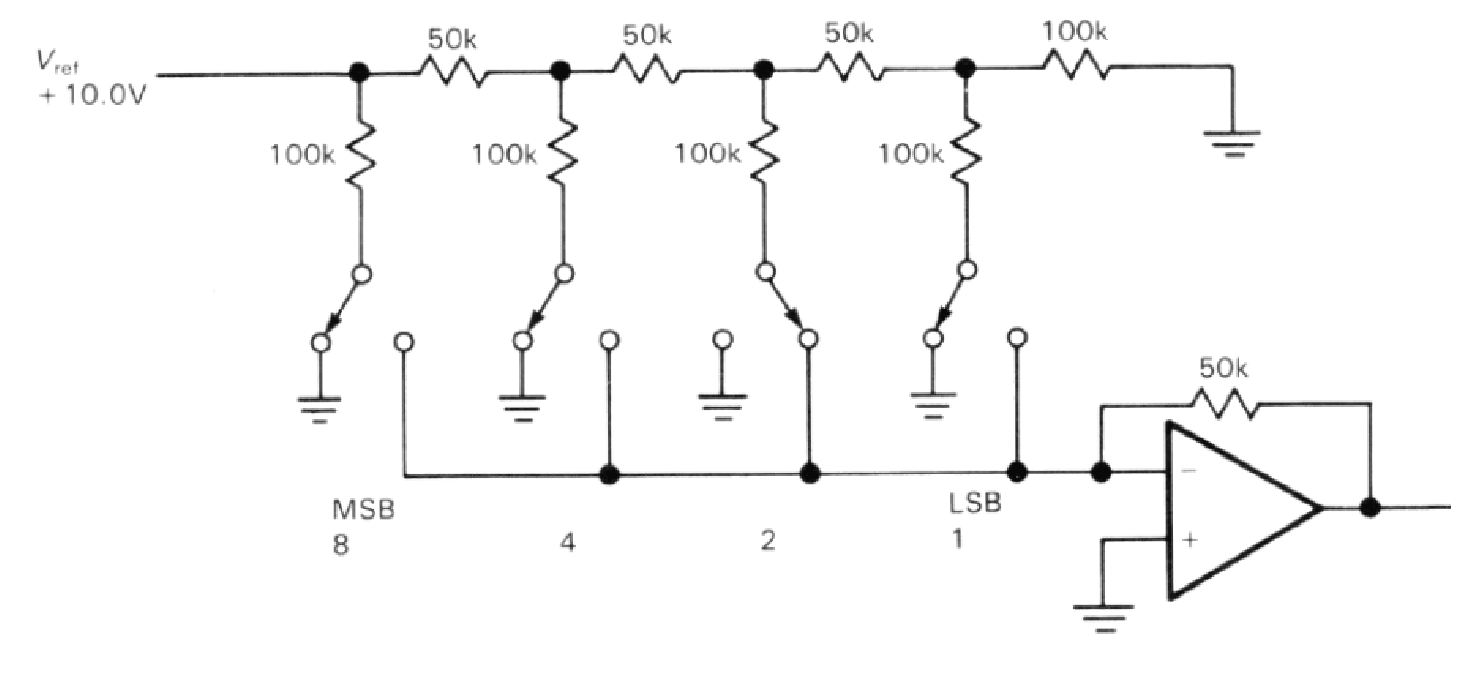
\includegraphics[width=0.75\linewidth]{DAC_R-2R/R-2R_DAC.eps}
\end{center}

\begin{itemize}
\item Solve for the currents through the 2R (100 k$\Omega$) resistors
associated with each bit branch for the binary numbers 1100 and 0011.  (A
switch will be in the GND position when it represents a `0'.)

\item How do the bit branch currents (1) compare to one another, and (2) change as a
function of the binary digit they represent (0 or 1)?  Does this make sense?

\item What is $V_o$ (the output voltage from the op amp) for the two binary numbers?
\end{itemize}
